\documentclass[12pt]{article}                   % Začátek dokumentu
\usepackage{../../MFFStyle}                     % Import stylu

\begin{document}
\begin{priklad}[5.1]
	Podrobně odvoďte a sestrojte přirozený kubický spline $S(x)$ interpolující funkci $f(x)$ danou tabulkou
	\begin{center}
		\begin{tabular}{|l|l|l|l|l|}
			\hline
			$i$      & 0 & 1 & 2 & 3 \\ \hline
			$x_i$    & 0 & 1 & 2 & 3 \\ \hline
			$f(x_i)$ & 0 & 1 & 0 & 0 \\ \hline
		\end{tabular}
	\end{center}
	Dále vypočtěte hodnotu $S(1.5)$.

	\begin{reseni}
		Jelikož chceme přirozený spline, tak $S''(x_0) = S''(x_3) = 0$. Z přednášky víme, že
		$$ \begin{pmatrix} 4 & 1 \\ 1 & 4 \end{pmatrix} \begin{pmatrix} S''(x_1) \\ S''(x_2) \end{pmatrix} = \begin{pmatrix} f(x_0) - 2f(x_1) + f(x_2) \\ f(x_1) - 2f(x_2) + f(x_3) \end{pmatrix} = \begin{pmatrix} -2 \\ 1 \end{pmatrix} $$
		Odečtením čtyřnásobku jedné rovnice od druhé získáme $S''(x_1) = -\frac{18}{5}$ a $S''(x_2) = \frac{12}{5}$. To pak můžeme dosadit do odvození z přednášky:{\tiny
		$$ S|_{[x_i, x_{i+1}]} = \frac{(x - x_i)^3}{6h}S''(x_{i+1}) + \frac{(x_{i+1} - x)^3}{6h}S''(x_i) + \(\frac{f(x_{i+1}) - f(x_i)}{h} - \frac{h}{6}\(S''(x_{i+1}) - S''(x_i)\)\)(x - x_i) + f(x_i) - \frac{h^2}{6}S''(x_i) $$
		$$ S|_{[0, 1]} = \frac{(x - 0)^3}{6·1}\(-\frac{18}{5}\) + \frac{(1 - x)^3}{6·1}0 + \(\frac{1 - 0}{1} - \frac{1}{6}\(-\frac{18}{5} - 0\)\)(x - 0) + 0 - \frac{1^2}{6}0 = \frac{8}{5}x - \frac{3}{5}x^3 $$
		$$ S|_{[1, 2]} = \frac{(x - 1)^3}{6·1}\frac{12}{5} + \frac{(2 - x)^3}{6·1}\(-\frac{18}{5}\) + \(\frac{0 - 1}{1} - \frac{1}{6}\(\frac{12}{5} + \frac{18}{5}\)\)(x - 1) + 1 - \frac{1^2}{6}\(-\frac{18}{5}\) = x^3 - \frac{24}{5}x^2 + \frac{32}{5}x - \frac{8}{5} $$
		$$ S|_{[2, 3]} = \frac{(x - 2)^3}{6·1}0 + \frac{(3 - x)^3}{6·1}\frac{12}{5} + \(\frac{0 - 0}{1} - \frac{1}{6}\(0 - \frac{12}{5}\)\)(x - 2) + 0 - \frac{1^2}{6}\frac{12}{5} = -\frac{2}{5}x^3 + \frac{18}{5}x^2 - \frac{52}{5}x + \frac{48}{5} $$
	}
		\begin{center}
			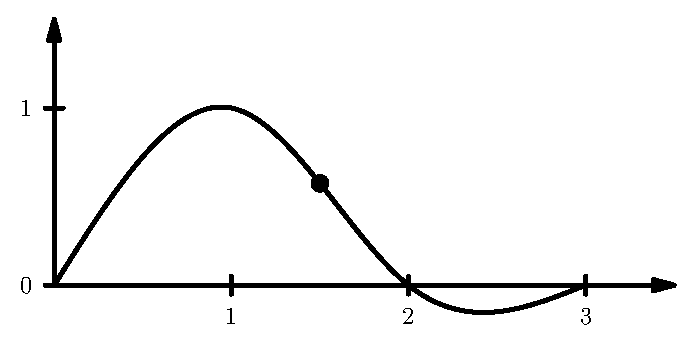
\includegraphics{spline.eps}
		\end{center}

		$$ S(1.5) = 1.5^3 - \frac{24}{5}1.5^2 + \frac{32}{5}1.5 - \frac{8}{5} = \frac{23}{40} = 0.575. $$
	\end{reseni}

	\begin{reseni}[Odvození]
		Jelikož máme málo bodů, můžeme hledat spline přímo (nemusíme zabíhat do obecného vzorce odvozeného pomocí Taylorova polynomu). Chceme kubický spline, tedy na jednotlivých intervalech bude druhá derivace lineární funkce. Navíc $S''(0) = 0 = S''(3)$, tedy jedinou možnost volby máme pro $S''(1)$ a $S''(2)$, volbou těchto dvou bude již $S''$ dáno. Tedy $S''|_{[0, 1]} = S''(1)x$, $S''|_{[1, 2]} = (x - 1) S''(2) - (x - 2)S''(1)$, $S''|_{[2, 3]} = -S''(2)(x - 3)$. Přidáním integrálu získáme:
		{\tiny $$ S'|_{[0, 1]} = \frac{x^2}{2} S''(1) + C_1, \qquad S'|_{[1, 2]} = \(\frac{x^2}{2} - x\) S''(2) - \(\frac{x^2}{2} - 2x\) S''(1) + C_2, \qquad S'|_{[2, 3]} = -\(\frac{x^2}{2} - 3x\)S''(2) + C_3. $$}%
		Spline má být $C^2([0, 3])$, tedy derivace zleva v bodě se rovná derivaci zprava. Pro body $1$ a $2$ je to tedy
		$$ \frac{1}{2} S''(1)x + C_1 = -\frac{1}{2} S''(2) + \frac{3}{2}S''(1) + C_2, \qquad 2S''(1) + C_2 = 4S''(2) + C_3. $$

		Druhým integrálem dosáhneme
		{\tiny $$ S|_{[0, 1]} = \frac{x^3}{6} S''(1) + C_1x + D_1, \qquad S|_{[1, 2]} = \(\frac{x^3}{6} - \frac{x^2}{2}\)S''(2) - \(\frac{x^3}{6} - x^2\) S''(1) + C_2x + D_2, \qquad S|_{[2, 3]} = -\(\frac{x^3}{6} - \frac{3x^2}{2}\)S''(2) + C_3 x + D_3. $$}%
		Víme, že přírůstek na prvním intervalu je $1$, na druhém $-1$ a na třetím $0$, tedy dosadíme krajní body a odečteme
		{\tiny $$ \frac{1}{6}S''(1) + C_1 = 1, \qquad \(-\frac{2}{3} + \frac{1}{3}\)S''(2) - \(- \frac{8}{3} + \frac{5}{6}\) S''(1) + C_2 = -1, \qquad -\(-9 + \frac{14}{3}\)S''(2) + C_3 = 0. $$}%
		Vyjádříme konstanty:
		$$ C_1 = 1 - \frac{1}{6} S''(1), \qquad C_2 = -1 + \frac{1}{3} S''(2) - \frac{11}{6} S''(1), \qquad C_3 = -\frac{13}{3} S''(2). $$
		A dosadím do podmínek daných rovnostmi prvních derivací:
		$$ 4S''(1) + S''(2) + 12 = 0, \quad S''(1) + 4S''(2) - 6 = 0 \quad \implies \quad S''(1) = -\frac{18}{5}, \quad S''(2) = \frac{12}{5}. $$
		Dosadíme zpět do konstant: $C_1 = \frac{8}{5}$, $C_2 = \frac{32}{5}$, $C_3 = -\frac{52}{5}$.

		Nyní můžeme vše dosadit do vyjádření $S$ a doplnit konstanty $D_i$ tak, aby spline procházela chtěnými body:
		$$ S(0) = D_1 = 0, \qquad S(1) = -\frac{4}{5} - 3 + \frac{32}{5} + D_2 = 1, \qquad S(2) = \frac{56}{5} - \frac{104}{5} + D_2 = 0 $$
		
		A získáme
		$$ S|_{[0, 1]} = \frac{8}{5}x - \frac{3}{5}x^3, \qquad S|_{[1, 2]} = x^3 - \frac{24}{5}x^2 + \frac{32}{5}x - \frac{8}{5}, \qquad S|_{[2, 3]} = -\frac{2}{5}x^3 + \frac{18}{5}x^2 - \frac{52}{5}x + \frac{48}{5}. $$
	\end{reseni}
\end{priklad}

\end{document}
